% Options for packages loaded elsewhere
\PassOptionsToPackage{unicode}{hyperref}
\PassOptionsToPackage{hyphens}{url}
%
\documentclass[
]{book}
\usepackage{amsmath,amssymb}
\usepackage{lmodern}
\usepackage{iftex}
\ifPDFTeX
  \usepackage[T1]{fontenc}
  \usepackage[utf8]{inputenc}
  \usepackage{textcomp} % provide euro and other symbols
\else % if luatex or xetex
  \usepackage{unicode-math}
  \defaultfontfeatures{Scale=MatchLowercase}
  \defaultfontfeatures[\rmfamily]{Ligatures=TeX,Scale=1}
\fi
% Use upquote if available, for straight quotes in verbatim environments
\IfFileExists{upquote.sty}{\usepackage{upquote}}{}
\IfFileExists{microtype.sty}{% use microtype if available
  \usepackage[]{microtype}
  \UseMicrotypeSet[protrusion]{basicmath} % disable protrusion for tt fonts
}{}
\makeatletter
\@ifundefined{KOMAClassName}{% if non-KOMA class
  \IfFileExists{parskip.sty}{%
    \usepackage{parskip}
  }{% else
    \setlength{\parindent}{0pt}
    \setlength{\parskip}{6pt plus 2pt minus 1pt}}
}{% if KOMA class
  \KOMAoptions{parskip=half}}
\makeatother
\usepackage{xcolor}
\usepackage{color}
\usepackage{fancyvrb}
\newcommand{\VerbBar}{|}
\newcommand{\VERB}{\Verb[commandchars=\\\{\}]}
\DefineVerbatimEnvironment{Highlighting}{Verbatim}{commandchars=\\\{\}}
% Add ',fontsize=\small' for more characters per line
\usepackage{framed}
\definecolor{shadecolor}{RGB}{248,248,248}
\newenvironment{Shaded}{\begin{snugshade}}{\end{snugshade}}
\newcommand{\AlertTok}[1]{\textcolor[rgb]{0.94,0.16,0.16}{#1}}
\newcommand{\AnnotationTok}[1]{\textcolor[rgb]{0.56,0.35,0.01}{\textbf{\textit{#1}}}}
\newcommand{\AttributeTok}[1]{\textcolor[rgb]{0.77,0.63,0.00}{#1}}
\newcommand{\BaseNTok}[1]{\textcolor[rgb]{0.00,0.00,0.81}{#1}}
\newcommand{\BuiltInTok}[1]{#1}
\newcommand{\CharTok}[1]{\textcolor[rgb]{0.31,0.60,0.02}{#1}}
\newcommand{\CommentTok}[1]{\textcolor[rgb]{0.56,0.35,0.01}{\textit{#1}}}
\newcommand{\CommentVarTok}[1]{\textcolor[rgb]{0.56,0.35,0.01}{\textbf{\textit{#1}}}}
\newcommand{\ConstantTok}[1]{\textcolor[rgb]{0.00,0.00,0.00}{#1}}
\newcommand{\ControlFlowTok}[1]{\textcolor[rgb]{0.13,0.29,0.53}{\textbf{#1}}}
\newcommand{\DataTypeTok}[1]{\textcolor[rgb]{0.13,0.29,0.53}{#1}}
\newcommand{\DecValTok}[1]{\textcolor[rgb]{0.00,0.00,0.81}{#1}}
\newcommand{\DocumentationTok}[1]{\textcolor[rgb]{0.56,0.35,0.01}{\textbf{\textit{#1}}}}
\newcommand{\ErrorTok}[1]{\textcolor[rgb]{0.64,0.00,0.00}{\textbf{#1}}}
\newcommand{\ExtensionTok}[1]{#1}
\newcommand{\FloatTok}[1]{\textcolor[rgb]{0.00,0.00,0.81}{#1}}
\newcommand{\FunctionTok}[1]{\textcolor[rgb]{0.00,0.00,0.00}{#1}}
\newcommand{\ImportTok}[1]{#1}
\newcommand{\InformationTok}[1]{\textcolor[rgb]{0.56,0.35,0.01}{\textbf{\textit{#1}}}}
\newcommand{\KeywordTok}[1]{\textcolor[rgb]{0.13,0.29,0.53}{\textbf{#1}}}
\newcommand{\NormalTok}[1]{#1}
\newcommand{\OperatorTok}[1]{\textcolor[rgb]{0.81,0.36,0.00}{\textbf{#1}}}
\newcommand{\OtherTok}[1]{\textcolor[rgb]{0.56,0.35,0.01}{#1}}
\newcommand{\PreprocessorTok}[1]{\textcolor[rgb]{0.56,0.35,0.01}{\textit{#1}}}
\newcommand{\RegionMarkerTok}[1]{#1}
\newcommand{\SpecialCharTok}[1]{\textcolor[rgb]{0.00,0.00,0.00}{#1}}
\newcommand{\SpecialStringTok}[1]{\textcolor[rgb]{0.31,0.60,0.02}{#1}}
\newcommand{\StringTok}[1]{\textcolor[rgb]{0.31,0.60,0.02}{#1}}
\newcommand{\VariableTok}[1]{\textcolor[rgb]{0.00,0.00,0.00}{#1}}
\newcommand{\VerbatimStringTok}[1]{\textcolor[rgb]{0.31,0.60,0.02}{#1}}
\newcommand{\WarningTok}[1]{\textcolor[rgb]{0.56,0.35,0.01}{\textbf{\textit{#1}}}}
\usepackage{longtable,booktabs,array}
\usepackage{calc} % for calculating minipage widths
% Correct order of tables after \paragraph or \subparagraph
\usepackage{etoolbox}
\makeatletter
\patchcmd\longtable{\par}{\if@noskipsec\mbox{}\fi\par}{}{}
\makeatother
% Allow footnotes in longtable head/foot
\IfFileExists{footnotehyper.sty}{\usepackage{footnotehyper}}{\usepackage{footnote}}
\makesavenoteenv{longtable}
\usepackage{graphicx}
\makeatletter
\def\maxwidth{\ifdim\Gin@nat@width>\linewidth\linewidth\else\Gin@nat@width\fi}
\def\maxheight{\ifdim\Gin@nat@height>\textheight\textheight\else\Gin@nat@height\fi}
\makeatother
% Scale images if necessary, so that they will not overflow the page
% margins by default, and it is still possible to overwrite the defaults
% using explicit options in \includegraphics[width, height, ...]{}
\setkeys{Gin}{width=\maxwidth,height=\maxheight,keepaspectratio}
% Set default figure placement to htbp
\makeatletter
\def\fps@figure{htbp}
\makeatother
\setlength{\emergencystretch}{3em} % prevent overfull lines
\providecommand{\tightlist}{%
  \setlength{\itemsep}{0pt}\setlength{\parskip}{0pt}}
\setcounter{secnumdepth}{5}
\usepackage{booktabs}
\ifLuaTeX
  \usepackage{selnolig}  % disable illegal ligatures
\fi
\usepackage[]{natbib}
\bibliographystyle{apalike}
\IfFileExists{bookmark.sty}{\usepackage{bookmark}}{\usepackage{hyperref}}
\IfFileExists{xurl.sty}{\usepackage{xurl}}{} % add URL line breaks if available
\urlstyle{same} % disable monospaced font for URLs
\hypersetup{
  pdftitle={Time-Series-Analysis},
  pdfauthor={shang-chieh0830},
  hidelinks,
  pdfcreator={LaTeX via pandoc}}

\title{Time-Series-Analysis}
\author{shang-chieh0830}
\date{2023-02-28}

\begin{document}
\maketitle

{
\setcounter{tocdepth}{1}
\tableofcontents
}
\hypertarget{about}{%
\chapter{About}\label{about}}

This book is a concise lecture note about \emph{Time Series Analysis}.

The content of this book is from the course Time Series Analysis taught by Chris Bilder. You can check his \href{https://www.youtube.com/@ChrisBilder}{YouTube channel} to get full(and correct) information about this course.

Again, I do \textbf{NOT} own the content of this book. I write this book only for studying. All credits belong to Chris Bilder.

If there is any copyright concerns, I will make this book private ASAP.

\hypertarget{introduction-to-r}{%
\chapter{Introduction to R}\label{introduction-to-r}}

We will go over some of the basic R operations in this section.

If you have questions, you should check \href{http://www.chrisbilder.com/stat878/sections.html}{Chris Bilder's website} for full information.

\hypertarget{basic-operation}{%
\section{Basic Operation}\label{basic-operation}}

\begin{Shaded}
\begin{Highlighting}[]
\DecValTok{2}\SpecialCharTok{+}\DecValTok{2}
\CommentTok{\#\textgreater{} [1] 4}
\end{Highlighting}
\end{Shaded}

\begin{Shaded}
\begin{Highlighting}[]
\DecValTok{2}\SpecialCharTok{\^{}}\DecValTok{3}
\CommentTok{\#\textgreater{} [1] 8}
\end{Highlighting}
\end{Shaded}

\begin{Shaded}
\begin{Highlighting}[]
\CommentTok{\# calculate the cdf of std. normal}
\FunctionTok{pnorm}\NormalTok{(}\FloatTok{1.96}\NormalTok{) }\CommentTok{\# 1.96 is the quantile}
\CommentTok{\#\textgreater{} [1] 0.9750021}
\end{Highlighting}
\end{Shaded}

\begin{Shaded}
\begin{Highlighting}[]
\FunctionTok{log}\NormalTok{(}\DecValTok{1}\NormalTok{)}
\CommentTok{\#\textgreater{} [1] 0}
\end{Highlighting}
\end{Shaded}

\begin{Shaded}
\begin{Highlighting}[]
\FunctionTok{sin}\NormalTok{(pi}\SpecialCharTok{/}\DecValTok{2}\NormalTok{)}
\CommentTok{\#\textgreater{} [1] 1}
\end{Highlighting}
\end{Shaded}

\begin{Shaded}
\begin{Highlighting}[]
\DecValTok{3}\SpecialCharTok{/}\DecValTok{4}
\CommentTok{\#\textgreater{} [1] 0.75}
\end{Highlighting}
\end{Shaded}

\begin{Shaded}
\begin{Highlighting}[]
\NormalTok{save }\OtherTok{\textless{}{-}} \DecValTok{2}\SpecialCharTok{+}\DecValTok{2}
\NormalTok{save}
\CommentTok{\#\textgreater{} [1] 4}
\end{Highlighting}
\end{Shaded}

\begin{Shaded}
\begin{Highlighting}[]
\FunctionTok{objects}\NormalTok{()}
\CommentTok{\#\textgreater{} [1] "save"}
\end{Highlighting}
\end{Shaded}

\begin{Shaded}
\begin{Highlighting}[]
\FunctionTok{ls}\NormalTok{()}
\CommentTok{\#\textgreater{} [1] "save"}
\end{Highlighting}
\end{Shaded}

\begin{Shaded}
\begin{Highlighting}[]
\CommentTok{\# quit operaiton}
\CommentTok{\# q() }
\end{Highlighting}
\end{Shaded}

\hypertarget{vectors}{%
\section{Vectors}\label{vectors}}

\begin{Shaded}
\begin{Highlighting}[]
\NormalTok{x }\OtherTok{\textless{}{-}} \FunctionTok{c}\NormalTok{(}\DecValTok{1}\NormalTok{,}\DecValTok{2}\NormalTok{,}\DecValTok{3}\NormalTok{,}\DecValTok{4}\NormalTok{,}\DecValTok{5}\NormalTok{)}
\NormalTok{x}
\CommentTok{\#\textgreater{} [1] 1 2 3 4 5}
\end{Highlighting}
\end{Shaded}

\begin{Shaded}
\begin{Highlighting}[]
\FunctionTok{sd}\NormalTok{(x)}
\CommentTok{\#\textgreater{} [1] 1.581139}
\end{Highlighting}
\end{Shaded}

\begin{Shaded}
\begin{Highlighting}[]
\NormalTok{mysd }\OtherTok{\textless{}{-}} \ControlFlowTok{function}\NormalTok{(x)\{}
  \FunctionTok{cat}\NormalTok{(}\StringTok{" My data }\SpecialCharTok{\textbackslash{}n}\StringTok{"}\NormalTok{, x, }\StringTok{"}\SpecialCharTok{\textbackslash{}n}\StringTok{ has std deviation"}\NormalTok{,}\FunctionTok{sqrt}\NormalTok{(}\FunctionTok{var}\NormalTok{(x)))}
\NormalTok{\}}


\FunctionTok{mysd}\NormalTok{(x)}
\CommentTok{\#\textgreater{}  My data }
\CommentTok{\#\textgreater{}  1 2 3 4 5 }
\CommentTok{\#\textgreater{}  has std deviation 1.581139}
\end{Highlighting}
\end{Shaded}

\begin{Shaded}
\begin{Highlighting}[]
\FunctionTok{pnorm}\NormalTok{(}\AttributeTok{q=}\FloatTok{1.96}\NormalTok{, }\AttributeTok{mean=}\FloatTok{1.96}\NormalTok{, }\AttributeTok{sd=}\DecValTok{1}\NormalTok{)}
\CommentTok{\#\textgreater{} [1] 0.5}
\end{Highlighting}
\end{Shaded}

The full syntax for \texttt{pnorm()} is \texttt{pnorm(q,\ mean\ =\ 0,\ sd\ =\ 1,\ lower.tail\ =\ TRUE,\ log.p\ =\ FALSE)}

\begin{Shaded}
\begin{Highlighting}[]
\FunctionTok{pnorm}\NormalTok{(}\AttributeTok{q=}\FunctionTok{c}\NormalTok{(}\SpecialCharTok{{-}}\FloatTok{1.96}\NormalTok{,}\FloatTok{1.96}\NormalTok{))}
\CommentTok{\#\textgreater{} [1] 0.0249979 0.9750021}
\end{Highlighting}
\end{Shaded}

\begin{Shaded}
\begin{Highlighting}[]
\NormalTok{x }\OtherTok{\textless{}{-}} \FunctionTok{c}\NormalTok{(}\FloatTok{3.68}\NormalTok{, }\SpecialCharTok{{-}}\FloatTok{3.63}\NormalTok{, }\FloatTok{0.80}\NormalTok{, }\FloatTok{3.03}\NormalTok{, }\SpecialCharTok{{-}}\FloatTok{9.86}\NormalTok{, }\SpecialCharTok{{-}}\FloatTok{8.66}\NormalTok{, }
    \SpecialCharTok{{-}}\FloatTok{2.38}\NormalTok{, }\FloatTok{8.94}\NormalTok{, }\FloatTok{0.52}\NormalTok{, }\FloatTok{1.25}\NormalTok{) }

\NormalTok{y }\OtherTok{\textless{}{-}} \FunctionTok{c}\NormalTok{(}\FloatTok{0.55}\NormalTok{, }\FloatTok{1.65}\NormalTok{, }\FloatTok{0.98}\NormalTok{, }\SpecialCharTok{{-}}\FloatTok{0.07}\NormalTok{, }\SpecialCharTok{{-}}\FloatTok{0.01}\NormalTok{, }\SpecialCharTok{{-}}\FloatTok{0.31}\NormalTok{, }
    \SpecialCharTok{{-}}\FloatTok{0.34}\NormalTok{, }\SpecialCharTok{{-}}\FloatTok{1.38}\NormalTok{, }\SpecialCharTok{{-}}\FloatTok{1.32}\NormalTok{, }\FloatTok{0.53}\NormalTok{)}

\NormalTok{x}\SpecialCharTok{+}\NormalTok{y}
\CommentTok{\#\textgreater{}  [1]  4.23 {-}1.98  1.78  2.96 {-}9.87 {-}8.97 {-}2.72  7.56 {-}0.80}
\CommentTok{\#\textgreater{} [10]  1.78}

\NormalTok{x}\SpecialCharTok{*}\NormalTok{y}
\CommentTok{\#\textgreater{}  [1]   2.0240  {-}5.9895   0.7840  {-}0.2121   0.0986   2.6846}
\CommentTok{\#\textgreater{}  [7]   0.8092 {-}12.3372  {-}0.6864   0.6625}
\end{Highlighting}
\end{Shaded}

\begin{Shaded}
\begin{Highlighting}[]
\FunctionTok{mean}\NormalTok{(x)}
\CommentTok{\#\textgreater{} [1] {-}0.631}
\NormalTok{x}\SpecialCharTok{{-}}\FunctionTok{mean}\NormalTok{(x)}
\CommentTok{\#\textgreater{}  [1]  4.311 {-}2.999  1.431  3.661 {-}9.229 {-}8.029 {-}1.749  9.571}
\CommentTok{\#\textgreater{}  [9]  1.151  1.881}

\NormalTok{x}\SpecialCharTok{*}\DecValTok{2}
\CommentTok{\#\textgreater{}  [1]   7.36  {-}7.26   1.60   6.06 {-}19.72 {-}17.32  {-}4.76  17.88}
\CommentTok{\#\textgreater{}  [9]   1.04   2.50}
\end{Highlighting}
\end{Shaded}

The element(elt)-wise operation makes our life easier.

\hypertarget{files}{%
\section{Files}\label{files}}

Click \href{http://www.chrisbilder.com/stat878/sections/1/gpa.csv}{gpa.csv} to download the GPA csv file.

Click \href{http://www.chrisbilder.com/stat878/sections/1/gpa.txt}{gpa.txt} to download the GPA txt file.

\begin{Shaded}
\begin{Highlighting}[]
\FunctionTok{getwd}\NormalTok{()}
\CommentTok{\#\textgreater{} [1] "/Users/weishangjie/Desktop/Time{-}Series{-}Analysis"}
\end{Highlighting}
\end{Shaded}

\begin{Shaded}
\begin{Highlighting}[]
\NormalTok{gpatxt }\OtherTok{\textless{}{-}} \FunctionTok{read.table}\NormalTok{(}\StringTok{"gpa.txt"}\NormalTok{, }\AttributeTok{header=}\ConstantTok{TRUE}\NormalTok{, }\AttributeTok{sep=}\StringTok{""}\NormalTok{)}
\NormalTok{gpacsv }\OtherTok{\textless{}{-}} \FunctionTok{read.csv}\NormalTok{(}\StringTok{"gpa.csv"}\NormalTok{)}
\end{Highlighting}
\end{Shaded}

\begin{Shaded}
\begin{Highlighting}[]
\NormalTok{gpacsv}\SpecialCharTok{$}\NormalTok{HSGPA}
\CommentTok{\#\textgreater{}  [1] 3.04 2.35 2.70 2.55 2.83 4.32 3.39 2.32 2.69 2.83 2.39}
\CommentTok{\#\textgreater{} [12] 3.65 2.85 3.83 2.22 1.98 2.88 4.00 2.28 2.88}
\end{Highlighting}
\end{Shaded}

\begin{Shaded}
\begin{Highlighting}[]
\NormalTok{gpacsv}\SpecialCharTok{$}\NormalTok{CollegeGPA}
\CommentTok{\#\textgreater{}  [1] 3.10 2.30 3.00 2.45 2.50 3.70 3.40 2.60 2.80 3.60 2.00}
\CommentTok{\#\textgreater{} [12] 2.90 3.30 3.20 2.80 2.40 2.60 3.80 2.20 2.60}
\end{Highlighting}
\end{Shaded}

\begin{Shaded}
\begin{Highlighting}[]
\NormalTok{gpacsv[}\DecValTok{1}\NormalTok{,}\DecValTok{1}\NormalTok{] }\CommentTok{\# [row, col]}
\CommentTok{\#\textgreater{} [1] 3.04}
\end{Highlighting}
\end{Shaded}

\begin{Shaded}
\begin{Highlighting}[]
\NormalTok{gpacsv[,}\DecValTok{1}\NormalTok{]}
\CommentTok{\#\textgreater{}  [1] 3.04 2.35 2.70 2.55 2.83 4.32 3.39 2.32 2.69 2.83 2.39}
\CommentTok{\#\textgreater{} [12] 3.65 2.85 3.83 2.22 1.98 2.88 4.00 2.28 2.88}
\end{Highlighting}
\end{Shaded}

\begin{Shaded}
\begin{Highlighting}[]
\NormalTok{gpacsv[}\FunctionTok{c}\NormalTok{(}\DecValTok{1}\NormalTok{,}\DecValTok{3}\NormalTok{,}\DecValTok{5}\NormalTok{),}\DecValTok{2}\NormalTok{]}
\CommentTok{\#\textgreater{} [1] 3.1 3.0 2.5}
\end{Highlighting}
\end{Shaded}

\begin{Shaded}
\begin{Highlighting}[]
\NormalTok{gpacsv[,}\StringTok{"HSGPA"}\NormalTok{]}
\CommentTok{\#\textgreater{}  [1] 3.04 2.35 2.70 2.55 2.83 4.32 3.39 2.32 2.69 2.83 2.39}
\CommentTok{\#\textgreater{} [12] 3.65 2.85 3.83 2.22 1.98 2.88 4.00 2.28 2.88}
\end{Highlighting}
\end{Shaded}

\begin{Shaded}
\begin{Highlighting}[]
\FunctionTok{summary}\NormalTok{(gpacsv)}
\CommentTok{\#\textgreater{}      HSGPA         CollegeGPA   }
\CommentTok{\#\textgreater{}  Min.   :1.980   Min.   :2.000  }
\CommentTok{\#\textgreater{}  1st Qu.:2.380   1st Qu.:2.487  }
\CommentTok{\#\textgreater{}  Median :2.830   Median :2.800  }
\CommentTok{\#\textgreater{}  Mean   :2.899   Mean   :2.862  }
\CommentTok{\#\textgreater{}  3rd Qu.:3.127   3rd Qu.:3.225  }
\CommentTok{\#\textgreater{}  Max.   :4.320   Max.   :3.800}
\end{Highlighting}
\end{Shaded}

\begin{Shaded}
\begin{Highlighting}[]
\FunctionTok{plot}\NormalTok{(}\AttributeTok{x =}\NormalTok{ gpacsv}\SpecialCharTok{$}\NormalTok{HSGPA, }\AttributeTok{y =}\NormalTok{ gpacsv}\SpecialCharTok{$}\NormalTok{CollegeGPA,}
     \AttributeTok{xlab =} \StringTok{"HS GPA"}\NormalTok{, }\AttributeTok{ylab =} \StringTok{"College GPA"}\NormalTok{, }
     \AttributeTok{main =} \StringTok{"College GPA vs. HS GPA"}\NormalTok{, }
     \AttributeTok{xlim =} \FunctionTok{c}\NormalTok{(}\DecValTok{0}\NormalTok{,}\FloatTok{4.5}\NormalTok{), }\AttributeTok{ylim =} \FunctionTok{c}\NormalTok{(}\DecValTok{0}\NormalTok{,}\FloatTok{4.5}\NormalTok{), }\AttributeTok{col =} \StringTok{"red"}\NormalTok{, }
    \AttributeTok{pch =} \DecValTok{1}\NormalTok{, }\AttributeTok{cex =} \FloatTok{1.0}\NormalTok{, }\AttributeTok{panel.first =} \FunctionTok{grid}\NormalTok{(}\AttributeTok{col =} \StringTok{"gray"}\NormalTok{, lty }
    \OtherTok{=} \StringTok{"dotted"}\NormalTok{))}
\end{Highlighting}
\end{Shaded}

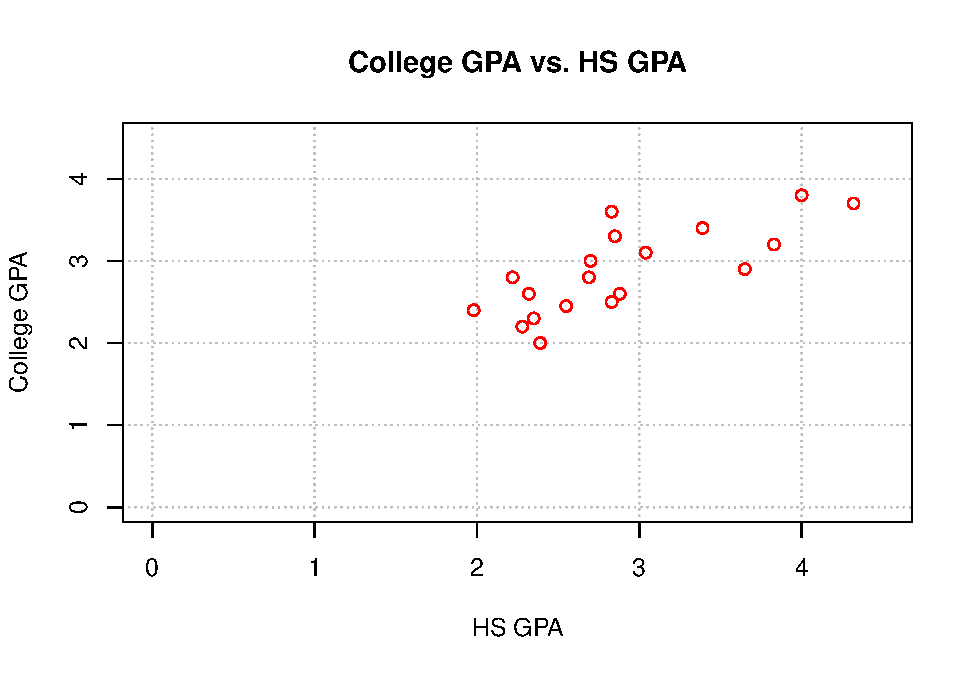
\includegraphics{01-Introduction-to-R_files/figure-latex/unnamed-chunk-27-1.pdf}
The \texttt{plot()} function creates a two dimensional plot of data.

Here are descriptions of its arguments:

\begin{itemize}
\item
  x specifies what is plotted for the x-axis.
\item
  y specifies what is plotted for the y-axis.
\item
  xlab and ylab specify the x-axis and y-axis labels, respectively.
\item
  main specifies the main title of the plot.
\item
  xlim and ylim specify the x-axis and y-axis limits, respectively.

  \begin{itemize}
  \tightlist
  \item
    Notice the use of the c() function.
  \end{itemize}
\item
  col specifies the color of the plotting points.

  \begin{itemize}
  \tightlist
  \item
    Run the \texttt{colors()} function to see what possible colors can be used.
  \item
    Also, you can see \href{https://github.com/EarlGlynn/colorchart/wiki/Color-Chart-in-R}{Here} for the colors from colors().
  \end{itemize}
\item
  \texttt{pch} specifies the plotting characters.
\item
  \texttt{cex}specifies the height of the plotting characters.
  The value 1.0 is the default.
\item
  \texttt{panel.first\ =\ grid()} specifies grid lines will be plotted.
\item
  The line types can be specified as follows:
  \texttt{1=solid,\ 2=dashed,\ 3=dotted,\ 4=dotdash,\ 5=longdash,\ 6=twodash} or as one of the character strings \texttt{"blank",\ "solid",\ "dashed",\ "dotted",\ \ "dotdash",\ "longdash"}, or \texttt{"twodash"}.\\
  These line type specifications can be used in other functions.\\
\item
  The \texttt{par()}(parameter) function's Help contains more information about the different plotting options!
\end{itemize}

\hypertarget{regression}{%
\section{Regression}\label{regression}}

Our is model is:\[CollegeGPA=\beta_0+\beta_1HSGPA+\epsilon\]

\begin{Shaded}
\begin{Highlighting}[]
\NormalTok{mod.fit }\OtherTok{\textless{}{-}} \FunctionTok{lm}\NormalTok{(}\AttributeTok{formula=}\NormalTok{ CollegeGPA}\SpecialCharTok{\textasciitilde{}}\NormalTok{ HSGPA, }\AttributeTok{data=}\NormalTok{gpacsv)}
\NormalTok{mod.fit}
\CommentTok{\#\textgreater{} }
\CommentTok{\#\textgreater{} Call:}
\CommentTok{\#\textgreater{} lm(formula = CollegeGPA \textasciitilde{} HSGPA, data = gpacsv)}
\CommentTok{\#\textgreater{} }
\CommentTok{\#\textgreater{} Coefficients:}
\CommentTok{\#\textgreater{} (Intercept)        HSGPA  }
\CommentTok{\#\textgreater{}      1.0869       0.6125}
\end{Highlighting}
\end{Shaded}

\begin{Shaded}
\begin{Highlighting}[]
\FunctionTok{names}\NormalTok{(mod.fit)}
\CommentTok{\#\textgreater{}  [1] "coefficients"  "residuals"     "effects"      }
\CommentTok{\#\textgreater{}  [4] "rank"          "fitted.values" "assign"       }
\CommentTok{\#\textgreater{}  [7] "qr"            "df.residual"   "xlevels"      }
\CommentTok{\#\textgreater{} [10] "call"          "terms"         "model"}
\end{Highlighting}
\end{Shaded}

\begin{Shaded}
\begin{Highlighting}[]
\NormalTok{mod.fit}\SpecialCharTok{$}\NormalTok{coefficients}
\CommentTok{\#\textgreater{} (Intercept)       HSGPA }
\CommentTok{\#\textgreater{}   1.0868795   0.6124941}
\end{Highlighting}
\end{Shaded}

\begin{Shaded}
\begin{Highlighting}[]
\FunctionTok{round}\NormalTok{(mod.fit}\SpecialCharTok{$}\NormalTok{residuals[}\DecValTok{1}\SpecialCharTok{:}\DecValTok{5}\NormalTok{],}\DecValTok{2}\NormalTok{)}
\CommentTok{\#\textgreater{}     1     2     3     4     5 }
\CommentTok{\#\textgreater{}  0.15 {-}0.23  0.26 {-}0.20 {-}0.32}
\end{Highlighting}
\end{Shaded}

\begin{Shaded}
\begin{Highlighting}[]
\FunctionTok{library}\NormalTok{(tidyverse)}
\CommentTok{\#\textgreater{} {-}{-} Attaching packages {-}{-}{-}{-}{-}{-}{-}{-}{-}{-}{-}{-}{-}{-}{-}{-}{-}{-}{-} tidyverse 1.3.2 {-}{-}}
\CommentTok{\#\textgreater{} v ggplot2 3.4.1     v purrr   1.0.1}
\CommentTok{\#\textgreater{} v tibble  3.1.8     v dplyr   1.1.0}
\CommentTok{\#\textgreater{} v tidyr   1.3.0     v stringr 1.5.0}
\CommentTok{\#\textgreater{} v readr   2.1.4     v forcats 0.5.2}
\CommentTok{\#\textgreater{} {-}{-} Conflicts {-}{-}{-}{-}{-}{-}{-}{-}{-}{-}{-}{-}{-}{-}{-}{-}{-}{-}{-}{-}{-}{-} tidyverse\_conflicts() {-}{-}}
\CommentTok{\#\textgreater{} x dplyr::filter() masks stats::filter()}
\CommentTok{\#\textgreater{} x dplyr::lag()    masks stats::lag()}
\NormalTok{save.fit }\OtherTok{\textless{}{-}} \FunctionTok{data.frame}\NormalTok{(gpacsv, }\AttributeTok{C.GPA.hat =} 
    \FunctionTok{round}\NormalTok{(mod.fit}\SpecialCharTok{$}\NormalTok{fitted.values,}\DecValTok{2}\NormalTok{), }\AttributeTok{residuals =} 
    \FunctionTok{round}\NormalTok{(mod.fit}\SpecialCharTok{$}\NormalTok{residuals,}\DecValTok{2}\NormalTok{))}

\NormalTok{save.fit }\SpecialCharTok{\%\textgreater{}\%} \FunctionTok{head}\NormalTok{()}
\CommentTok{\#\textgreater{}   HSGPA CollegeGPA C.GPA.hat residuals}
\CommentTok{\#\textgreater{} 1  3.04       3.10      2.95      0.15}
\CommentTok{\#\textgreater{} 2  2.35       2.30      2.53     {-}0.23}
\CommentTok{\#\textgreater{} 3  2.70       3.00      2.74      0.26}
\CommentTok{\#\textgreater{} 4  2.55       2.45      2.65     {-}0.20}
\CommentTok{\#\textgreater{} 5  2.83       2.50      2.82     {-}0.32}
\CommentTok{\#\textgreater{} 6  4.32       3.70      3.73     {-}0.03}
\end{Highlighting}
\end{Shaded}

\begin{Shaded}
\begin{Highlighting}[]
\FunctionTok{summary}\NormalTok{(mod.fit)}
\CommentTok{\#\textgreater{} }
\CommentTok{\#\textgreater{} Call:}
\CommentTok{\#\textgreater{} lm(formula = CollegeGPA \textasciitilde{} HSGPA, data = gpacsv)}
\CommentTok{\#\textgreater{} }
\CommentTok{\#\textgreater{} Residuals:}
\CommentTok{\#\textgreater{}      Min       1Q   Median       3Q      Max }
\CommentTok{\#\textgreater{} {-}0.55074 {-}0.25086  0.01633  0.24242  0.77976 }
\CommentTok{\#\textgreater{} }
\CommentTok{\#\textgreater{} Coefficients:}
\CommentTok{\#\textgreater{}             Estimate Std. Error t value Pr(\textgreater{}|t|)    }
\CommentTok{\#\textgreater{} (Intercept)   1.0869     0.3666   2.965 0.008299 ** }
\CommentTok{\#\textgreater{} HSGPA         0.6125     0.1237   4.953 0.000103 ***}
\CommentTok{\#\textgreater{} {-}{-}{-}}
\CommentTok{\#\textgreater{} Signif. codes:  }
\CommentTok{\#\textgreater{} 0 \textquotesingle{}***\textquotesingle{} 0.001 \textquotesingle{}**\textquotesingle{} 0.01 \textquotesingle{}*\textquotesingle{} 0.05 \textquotesingle{}.\textquotesingle{} 0.1 \textquotesingle{} \textquotesingle{} 1}
\CommentTok{\#\textgreater{} }
\CommentTok{\#\textgreater{} Residual standard error: 0.3437 on 18 degrees of freedom}
\CommentTok{\#\textgreater{} Multiple R{-}squared:  0.5768, Adjusted R{-}squared:  0.5533 }
\CommentTok{\#\textgreater{} F{-}statistic: 24.54 on 1 and 18 DF,  p{-}value: 0.0001027}
\end{Highlighting}
\end{Shaded}

Hence, our estimated regression model is\[ \hat{collge.GPA}=\hat{\beta_0}+\hat{\beta_1}HS.GPA
=1.0869+0.6125HS.GPA\]

\begin{Shaded}
\begin{Highlighting}[]
\CommentTok{\# Open a new graphics window }
\CommentTok{\# device new}
\FunctionTok{dev.new}\NormalTok{(}\AttributeTok{width =} \DecValTok{8}\NormalTok{, }\AttributeTok{height =} \DecValTok{6}\NormalTok{, }\AttributeTok{pointsize =} \DecValTok{10}\NormalTok{)}


\CommentTok{\# 1 row and 2 columns of plots}
\FunctionTok{par}\NormalTok{(}\AttributeTok{mfrow =} \FunctionTok{c}\NormalTok{(}\DecValTok{1}\NormalTok{,}\DecValTok{2}\NormalTok{))}
\CommentTok{\# par= graphic parameter}
\CommentTok{\# mfrow= make a frame by row}

\CommentTok{\# Same scatter plot as before}
\FunctionTok{plot}\NormalTok{(}\AttributeTok{x =}\NormalTok{ gpacsv}\SpecialCharTok{$}\NormalTok{HSGPA, }\AttributeTok{y =}\NormalTok{ gpacsv}\SpecialCharTok{$}\NormalTok{CollegeGPA, }\AttributeTok{xlab =} \StringTok{"HS }
\StringTok{    GPA"}\NormalTok{, }\AttributeTok{ylab =} \StringTok{"College GPA"}\NormalTok{, }\AttributeTok{main =} \StringTok{"College GPA vs. }
\StringTok{    HS GPA"}\NormalTok{, }\AttributeTok{xlim =} \FunctionTok{c}\NormalTok{(}\DecValTok{0}\NormalTok{,}\FloatTok{4.5}\NormalTok{), }\AttributeTok{ylim =} \FunctionTok{c}\NormalTok{(}\DecValTok{0}\NormalTok{,}\FloatTok{4.5}\NormalTok{), }\AttributeTok{col =} 
    \StringTok{"red"}\NormalTok{, }\AttributeTok{pch =} \DecValTok{1}\NormalTok{, }\AttributeTok{cex =} \FloatTok{1.0}\NormalTok{, }\AttributeTok{panel.first =} \FunctionTok{grid}\NormalTok{(}\AttributeTok{col =} 
    \StringTok{"gray"}\NormalTok{, }\AttributeTok{lty =} \StringTok{"dotted"}\NormalTok{))}
    
\CommentTok{\# Puts the line y = a + bx on the plot}
\FunctionTok{abline}\NormalTok{(}\AttributeTok{a =}\NormalTok{ mod.fit}\SpecialCharTok{$}\NormalTok{coefficients[}\DecValTok{1}\NormalTok{], }\AttributeTok{b =} 
\NormalTok{    mod.fit}\SpecialCharTok{$}\NormalTok{coefficients[}\DecValTok{2}\NormalTok{], }\AttributeTok{lty =} \StringTok{"solid"}\NormalTok{, }\AttributeTok{col =} 
    \StringTok{"blue"}\NormalTok{, }\AttributeTok{lwd =} \DecValTok{2}\NormalTok{)}
    

\CommentTok{\# Same scatter plot as before}
\FunctionTok{plot}\NormalTok{(}\AttributeTok{x =}\NormalTok{ gpacsv}\SpecialCharTok{$}\NormalTok{HSGPA, }\AttributeTok{y =}\NormalTok{ gpacsv}\SpecialCharTok{$}\NormalTok{CollegeGPA, }\AttributeTok{xlab =} \StringTok{"HS }
\StringTok{    GPA"}\NormalTok{, }\AttributeTok{ylab =} \StringTok{"College GPA"}\NormalTok{, }\AttributeTok{main =} \StringTok{"College GPA vs. }
\StringTok{    HS GPA"}\NormalTok{, }\AttributeTok{xlim =} \FunctionTok{c}\NormalTok{(}\DecValTok{0}\NormalTok{,}\FloatTok{4.5}\NormalTok{), }\AttributeTok{ylim =} \FunctionTok{c}\NormalTok{(}\DecValTok{0}\NormalTok{,}\FloatTok{4.5}\NormalTok{), }\AttributeTok{col =} 
    \StringTok{"red"}\NormalTok{, }\AttributeTok{pch =} \DecValTok{1}\NormalTok{, }\AttributeTok{cex =} \FloatTok{1.0}\NormalTok{, }\AttributeTok{panel.first =} \FunctionTok{grid}\NormalTok{(}\AttributeTok{col =} 
    \StringTok{"gray"}\NormalTok{, }\AttributeTok{lty =} \StringTok{"dotted"}\NormalTok{))}


\CommentTok{\# Add line}
\CommentTok{\# expr= math expression}
\FunctionTok{curve}\NormalTok{(}\AttributeTok{expr =}\NormalTok{ mod.fit}\SpecialCharTok{$}\NormalTok{coefficients[}\DecValTok{1}\NormalTok{] }\SpecialCharTok{+} 
\NormalTok{    mod.fit}\SpecialCharTok{$}\NormalTok{coefficients[}\DecValTok{2}\NormalTok{]}\SpecialCharTok{*}\NormalTok{x, }
    \AttributeTok{xlim =} \FunctionTok{c}\NormalTok{(}\FunctionTok{min}\NormalTok{(gpacsv}\SpecialCharTok{$}\NormalTok{HSGPA),}\FunctionTok{max}\NormalTok{(gpacsv}\SpecialCharTok{$}\NormalTok{HSGPA)), }
    \AttributeTok{col=} \StringTok{"blue"}\NormalTok{, }\AttributeTok{add =} \ConstantTok{TRUE}\NormalTok{, }\AttributeTok{lwd =} \DecValTok{2}\NormalTok{)}
\end{Highlighting}
\end{Shaded}

\begin{itemize}
\item
  The \texttt{dev.new()} function can be used to open a new plotting window.
\item
  The \texttt{abline()} function can be used to draw straight lines on a plot. In the format used here, the line y = a + bx was drawn where a was the (intercept) and b was the (slope).
\item
  In the second plot, the curve() function was used to draw the line on the plot. This was done to have the line within the range of the high school GPA values.
\end{itemize}

Let's use function to automate what we have done.

\begin{Shaded}
\begin{Highlighting}[]
\NormalTok{my.reg.func }\OtherTok{\textless{}{-}} \ControlFlowTok{function}\NormalTok{(x, y, data) \{}

    \CommentTok{\# Fit the simple linear regression model and save the results in mod.fit}
\NormalTok{    mod.fit }\OtherTok{\textless{}{-}} \FunctionTok{lm}\NormalTok{(}\AttributeTok{formula =}\NormalTok{ y }\SpecialCharTok{\textasciitilde{}}\NormalTok{ x, }\AttributeTok{data =}\NormalTok{ data)}

    \CommentTok{\#Open a new graphics window {-} do not need to}
    \FunctionTok{dev.new}\NormalTok{(}\AttributeTok{width =} \DecValTok{6}\NormalTok{, }\AttributeTok{height =} \DecValTok{6}\NormalTok{, }\AttributeTok{pointsize =} \DecValTok{10}\NormalTok{)}

    \CommentTok{\# Same scatter plot as before}
    \FunctionTok{plot}\NormalTok{(}\AttributeTok{x =}\NormalTok{ x, }\AttributeTok{y =}\NormalTok{ y, }\AttributeTok{xlab =} \StringTok{"x"}\NormalTok{, }\AttributeTok{ylab =} \StringTok{"y"}\NormalTok{, }\AttributeTok{main =} \StringTok{"y vs. x"}\NormalTok{, }\AttributeTok{panel.first=}\FunctionTok{grid}\NormalTok{(}\AttributeTok{col =} \StringTok{"gray"}\NormalTok{, }\AttributeTok{lty =} 
      \StringTok{"dotted"}\NormalTok{))}

    \CommentTok{\# Plot model}
    \FunctionTok{curve}\NormalTok{(}\AttributeTok{expr =}\NormalTok{ mod.fit}\SpecialCharTok{$}\NormalTok{coefficients[}\DecValTok{1}\NormalTok{] }\SpecialCharTok{+} 
\NormalTok{      mod.fit}\SpecialCharTok{$}\NormalTok{coefficients[}\DecValTok{2}\NormalTok{]}\SpecialCharTok{*}\NormalTok{x, }\AttributeTok{xlim =} \FunctionTok{c}\NormalTok{(}\FunctionTok{min}\NormalTok{(x),}\FunctionTok{max}\NormalTok{(x)), }
      \AttributeTok{col =} \StringTok{"blue"}\NormalTok{, }\AttributeTok{add =} \ConstantTok{TRUE}\NormalTok{)}

    \CommentTok{\# This is the object returned}
\NormalTok{    mod.fit}
\NormalTok{  \}}
\end{Highlighting}
\end{Shaded}

\begin{Shaded}
\begin{Highlighting}[]
\NormalTok{save.it }\OtherTok{\textless{}{-}} \FunctionTok{my.reg.func}\NormalTok{(}\AttributeTok{x =}\NormalTok{ gpacsv}\SpecialCharTok{$}\NormalTok{HSGPA, }\AttributeTok{y =} 
\NormalTok{    gpacsv}\SpecialCharTok{$}\NormalTok{CollegeGPA, }\AttributeTok{data =}\NormalTok{ gpacsv)}
\end{Highlighting}
\end{Shaded}

To get specific x-axis or y-axis tick marks on a plot, use the \texttt{axis()} function. For example,

\begin{Shaded}
\begin{Highlighting}[]
\CommentTok{\#Note that xaxt = "n" tells R to not give any labels on the }
\CommentTok{\#  x{-}axis (yaxt = "n" works for y{-}axis)}
\FunctionTok{plot}\NormalTok{(}\AttributeTok{x =}\NormalTok{ gpacsv}\SpecialCharTok{$}\NormalTok{HSGPA, }\AttributeTok{y =}\NormalTok{ gpacsv}\SpecialCharTok{$}\NormalTok{CollegeGPA, }\AttributeTok{xlab =} \StringTok{"HS GPA"}\NormalTok{, }
     \AttributeTok{ylab =} \StringTok{"College GPA"}\NormalTok{, }\AttributeTok{main =} \StringTok{"College GPA vs. HS GPA"}\NormalTok{, }
     \AttributeTok{xaxt =} \StringTok{"n"}\NormalTok{, }\AttributeTok{xlim =} \FunctionTok{c}\NormalTok{(}\DecValTok{0}\NormalTok{, }\FloatTok{4.5}\NormalTok{), }\AttributeTok{ylim =} \FunctionTok{c}\NormalTok{(}\DecValTok{0}\NormalTok{, }\FloatTok{4.5}\NormalTok{), }\AttributeTok{col =} 
     \StringTok{"red"}\NormalTok{, }\AttributeTok{pch =} \DecValTok{1}\NormalTok{)}
\end{Highlighting}
\end{Shaded}

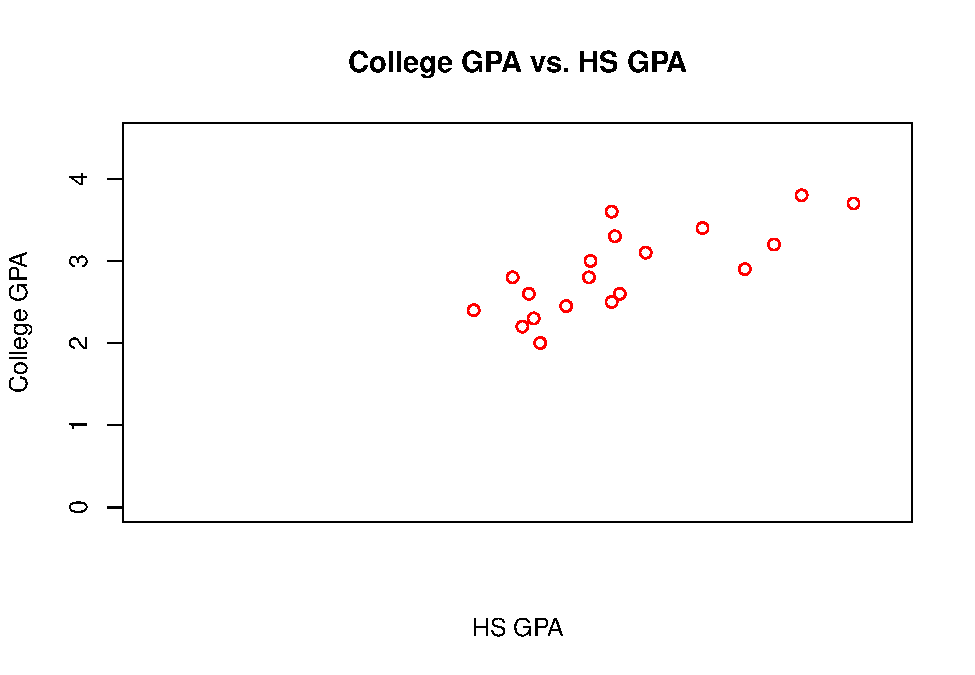
\includegraphics{01-Introduction-to-R_files/figure-latex/unnamed-chunk-37-1.pdf}

\begin{Shaded}
\begin{Highlighting}[]
\FunctionTok{plot}\NormalTok{(}\AttributeTok{x =}\NormalTok{ gpacsv}\SpecialCharTok{$}\NormalTok{HSGPA, }\AttributeTok{y =}\NormalTok{ gpacsv}\SpecialCharTok{$}\NormalTok{CollegeGPA, }\AttributeTok{xlab =} \StringTok{"HS GPA"}\NormalTok{, }
     \AttributeTok{ylab =} \StringTok{"College GPA"}\NormalTok{, }\AttributeTok{main =} \StringTok{"College GPA vs. HS GPA"}\NormalTok{, }
     \AttributeTok{xaxt =} \StringTok{"n"}\NormalTok{, }\AttributeTok{xlim =} \FunctionTok{c}\NormalTok{(}\DecValTok{0}\NormalTok{, }\FloatTok{4.5}\NormalTok{), }\AttributeTok{ylim =} \FunctionTok{c}\NormalTok{(}\DecValTok{0}\NormalTok{, }\FloatTok{4.5}\NormalTok{), }\AttributeTok{col =} 
     \StringTok{"red"}\NormalTok{, }\AttributeTok{pch =} \DecValTok{1}\NormalTok{)}
     
\CommentTok{\#Major tick marks}
\FunctionTok{axis}\NormalTok{(}\AttributeTok{side =} \DecValTok{1}\NormalTok{, }\AttributeTok{at =} \FunctionTok{seq}\NormalTok{(}\AttributeTok{from =} \DecValTok{0}\NormalTok{, }\AttributeTok{to =} \FloatTok{4.5}\NormalTok{, }\AttributeTok{by =} \FloatTok{0.5}\NormalTok{)) }
\end{Highlighting}
\end{Shaded}

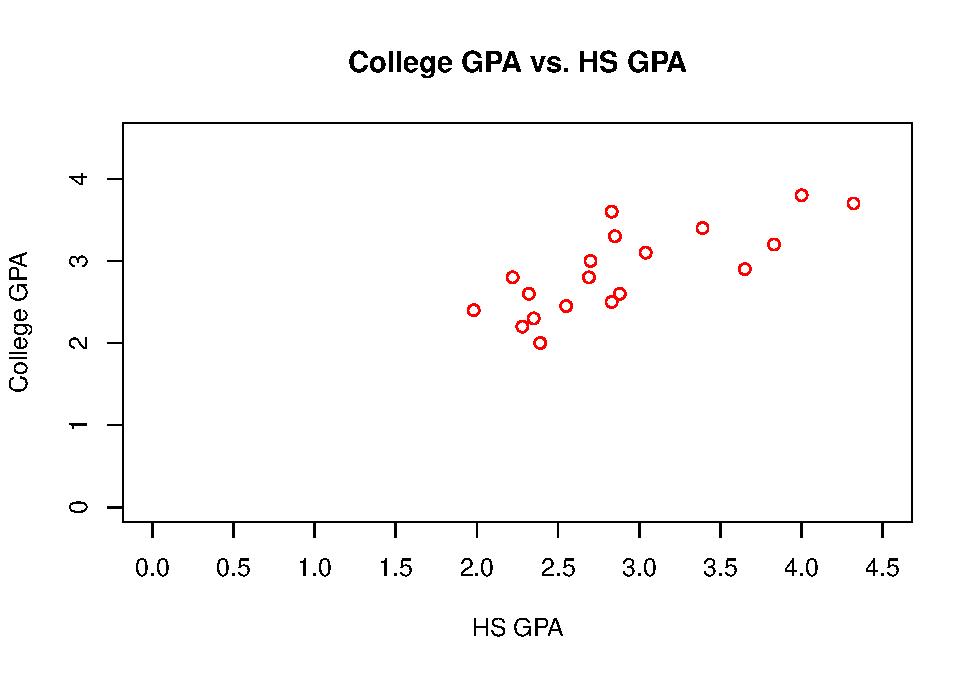
\includegraphics{01-Introduction-to-R_files/figure-latex/unnamed-chunk-38-1.pdf}

\begin{Shaded}
\begin{Highlighting}[]
\FunctionTok{plot}\NormalTok{(}\AttributeTok{x =}\NormalTok{ gpacsv}\SpecialCharTok{$}\NormalTok{HSGPA, }\AttributeTok{y =}\NormalTok{ gpacsv}\SpecialCharTok{$}\NormalTok{CollegeGPA, }\AttributeTok{xlab =} \StringTok{"HS GPA"}\NormalTok{, }
     \AttributeTok{ylab =} \StringTok{"College GPA"}\NormalTok{, }\AttributeTok{main =} \StringTok{"College GPA vs. HS GPA"}\NormalTok{, }
     \AttributeTok{xaxt =} \StringTok{"n"}\NormalTok{, }\AttributeTok{xlim =} \FunctionTok{c}\NormalTok{(}\DecValTok{0}\NormalTok{, }\FloatTok{4.5}\NormalTok{), }\AttributeTok{ylim =} \FunctionTok{c}\NormalTok{(}\DecValTok{0}\NormalTok{, }\FloatTok{4.5}\NormalTok{), }\AttributeTok{col =} 
     \StringTok{"red"}\NormalTok{, }\AttributeTok{pch =} \DecValTok{1}\NormalTok{)}
     
\CommentTok{\#Major tick marks}
\FunctionTok{axis}\NormalTok{(}\AttributeTok{side =} \DecValTok{1}\NormalTok{, }\AttributeTok{at =} \FunctionTok{seq}\NormalTok{(}\AttributeTok{from =} \DecValTok{0}\NormalTok{, }\AttributeTok{to =} \FloatTok{4.5}\NormalTok{, }\AttributeTok{by =} \FloatTok{0.5}\NormalTok{)) }

\CommentTok{\#Minor tick marks}
\FunctionTok{axis}\NormalTok{(}\AttributeTok{side =} \DecValTok{1}\NormalTok{, }\AttributeTok{at =} \FunctionTok{seq}\NormalTok{(}\AttributeTok{from =} \DecValTok{0}\NormalTok{, }\AttributeTok{to =} \FloatTok{4.5}\NormalTok{, }\AttributeTok{by =} \FloatTok{0.1}\NormalTok{), tck }
      \OtherTok{=} \FloatTok{0.01}\NormalTok{, }\AttributeTok{labels =} \ConstantTok{FALSE}\NormalTok{) }
\end{Highlighting}
\end{Shaded}

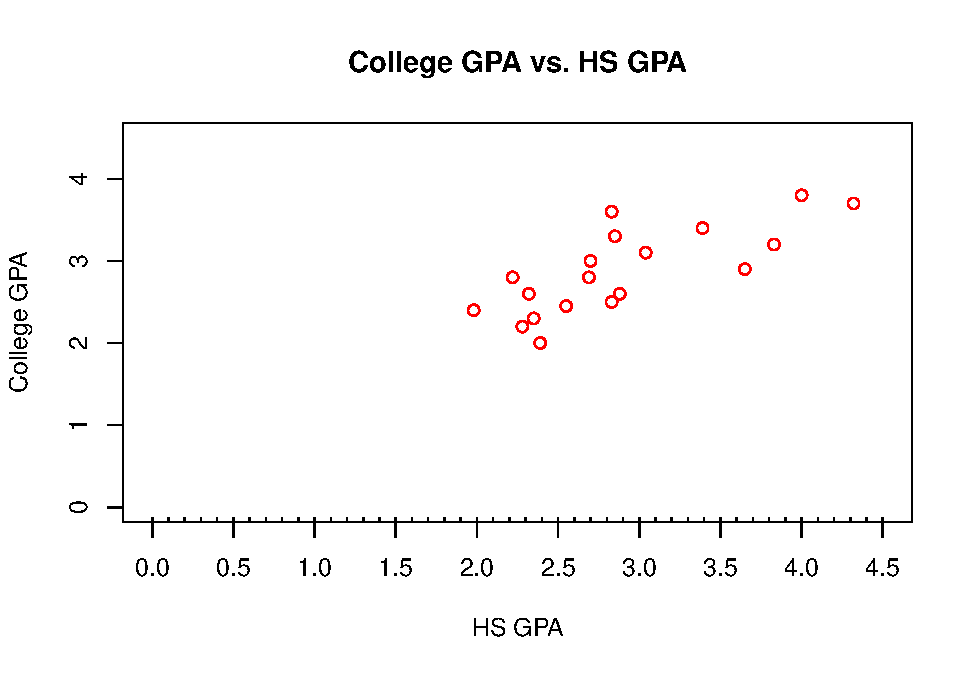
\includegraphics{01-Introduction-to-R_files/figure-latex/unnamed-chunk-39-1.pdf}

  \bibliography{book.bib,packages.bib}

\end{document}
